% Test tex file!

\documentclass[a4paper,12pt]{article}
\usepackage{times}  % DO NOT CHANGE THIS
\usepackage{helvet} % DO NOT CHANGE THIS
\usepackage{courier}  % DO NOT CHANGE THIS
\usepackage[hyphens]{url}  % DO NOT CHANGE THIS
\usepackage{graphicx} % DO NOT CHANGE THIS
\urlstyle{rm} % DO NOT CHANGE THIS
\def\UrlFont{\rm}  % DO NOT CHANGE THIS
\usepackage{natbib}  % DO NOT CHANGE THIS AND DO NOT ADD ANY OPTIONS TO IT
\usepackage[font=scriptsize]{caption} % DO NOT CHANGE THIS AND DO NOT ADD ANY OPTIONS TO IT
\frenchspacing  % DO NOT CHANGE THIS
\setlength{\pdfpagewidth}{8.5in}  % DO NOT CHANGE THIS
\setlength{\pdfpageheight}{11in}  % DO NOT CHANGE THIS
\usepackage{algorithm} %format of the algorithm 
\usepackage{algorithmic} %format of the algorithm 
\usepackage{multirow} %multirow for format of table 
\usepackage{amsmath} 
\usepackage{xcolor}
\usepackage{amssymb}
\usepackage{amsmath}
\usepackage{CJKutf8}
\usepackage{courier}
\begin{document}

\begin{CJK}{UTF8}{gbsn}
% \begin{CJK}{UTF8}{gkai}

\title{强化学习:作业二}

\author{傅浩敏 MG20370012}

\date{2020年11月14日}

\maketitle

\section{作业内容}
在gridworld环境中实现Q-learning算法。本实验的gridworld是一个8*8的迷宫,游戏开始时会随机初始化当前位置,游戏目标是到达迷宫终点。在行动过程中,每走一步会减少1点奖励,到达终点后可以获得100点的奖励。我们需要使用Q-learning算法在不同位置做出决策,使得游戏结束时获得最大的奖励。由于游戏初始位置随机生成,因此并非每次都能取得最大的奖励,只有当初始位置恰好在终点旁边时才有可能获得99点最大奖励,如Figure 1和Figure 2,当初始位置在Figure 3处时最多只能获得85点奖励。
\begin{figure}[htbp]
	\centering
	\begin{minipage}[t]{0.25\textwidth}
		\centering
		
\includegraphics[width=2cm]{code/obs_1.jpeg}
		\caption{最佳情况}
	\end{minipage}
	\begin{minipage}[t]{0.25\textwidth}
		\centering
		
\includegraphics[width=2cm]{code/obs_2.jpeg}
		\caption{最佳情况}
	\end{minipage}
	\begin{minipage}[t]{0.25\textwidth}
		\centering
		
\includegraphics[width=2cm]{code/obs_3.jpeg}
		\caption{最坏情况}
	\end{minipage}
\end{figure}

\section{实现过程}
\subsection{算法描述}
首先在 \texttt{algo.py} 中实现 \texttt{Q-learning Agent},我们需要在 \texttt{Agent} 中维护一个关于策略 $\pi$ 在状态 $s$ 下执行动作 $a$ 的长期回报 $Q_\pi(s,a)$ 的表格。\texttt{Agent} 在状态 $s$ 下会选取使 $Q_\pi(s,a)$ 最大的动作 $a$。每次选取并执行完一批动作后,我们需要以下式更新表格中长期回报的值:
$$
\begin{cases}
		&a'= \mathop{\arg\max}_{x} Q_\pi(s',x)\\
		&Q_\pi(s,a)=Q_\pi(s,a)+\alpha(r+\gamma Q_\pi(s',a')-Q_\pi(s,a)) 
\end{cases}
$$
其中 $s'$ 是在状态 $s$ 下执行动作 $a$ 后的新状态,$\alpha$ 和 $\gamma$ 分别为学习率和折扣系数。迭代此过程可以使长期回报 $Q_\pi(s,a)$ 逐步逼近在 $s$ 位置上选取不同动作的真实长期回报的相对值(考虑折扣),从而在不同位置做出合理的选择。


模型在训练过程中采用 Epsilon-Greedy 算法,在环境中采样时会有一定的概率随机选取动作,但在预测时会关闭探索。模型在采样若干个状态对后再统一更新长期回报表 $Q_\pi(s,a)$,并重复此过程。


模型加入了经验回放机制,\texttt{Agent} 会维护一个关于四元组 $(s,a,s',r)$ 的经验回放池。在每次更新长期回报时,模型会同时迭代当前的动作选择和经验回放池中保存的状态,在更新完成后,若回放池未满则直接将当前动作选择对应的四元组放入,否则随机选择池中一个四元组进行替换。
\subsection{代码实现}
我采用了动态扩展的方式维护长期回报表 $Q_\pi$ ,每次访问 $Q_\pi$ 时,如果访问状态 $s$ 不存在,则初始化 $Q_\pi(s)$。$\pi(s)$ 会选取使 $Q_\pi(s)$ 最大的动作 $a$,$\pi_\epsilon(s)$ 则会在此基础上以 $\epsilon$ 的概率随机选择动作。因此训练的大致过程如下:
\begin{algorithm}[!h]
	\caption{Q-learning Training}
	\begin{algorithmic}[1]
		\STATE initial $Q_\pi,replay\_pool$
		\FOR{$1,2,\cdots$}
		\STATE initial $samples,env$
		\STATE $s=$ observation of $env$
			\FOR{$1,\cdots,steps$}
			\STATE $a=\pi_\epsilon(s)$
			\STATE $s',r=$ do action $a$ on $env$
			\STATE $sapmles.append(s,a,s',r)$
			\STATE $s=s'$
			\ENDFOR
			\FOR{$(s,a,s',r)$ in $sapmles$}
			\STATE $a'=\pi(s')$
			\STATE $Q_\pi(s,a)=Q_\pi(s,a)+\alpha(r+\gamma Q_\pi(s',a')-Q_\pi(s,a))$
				\FOR{$(rs,ra,rs',rr)$ in $replay\_pool$}
					\STATE $ra'=\pi(rs')$
					\STATE $Q_\pi(rs,ra)=Q_\pi(rs,ra)+\alpha(rr+\gamma Q_\pi(rs',ra')-Q_\pi(rs,ra))$
				\ENDFOR
			\STATE $replay\_pool.update(s,a,s',r)$
			\ENDFOR
		\ENDFOR
	\end{algorithmic}
\end{algorithm}
\section{复现方式}
\subsection{结果复现}
首先在主文件夹下运行 \texttt{pip install -r requirements.txt} 安装依赖,如果已安装依赖也可跳过此步骤。然后需要在 \texttt{code} 文件夹下运行 \texttt{python main.py} 开始实验。实验结果保存为 performance.png ,直接运行的结果在默认参数下进行,可以获得与 Figure 4 类似的效果。如果希望获得对比实验中的效果,则需要修改部分参数,具体参数内容在3.2节进行说明。
\subsection{参数介绍}
\begin{table}[!h]
	\renewcommand{\arraystretch}{1.1}
	\caption{自定义运行参数}
	\centering
	\begin{tabular}{ccc}
		\hline
		名称& 默认值& 说明\\
		\hline
		--batch-update& True & 是否批量更新$Q_\pi$\\
		--auto-learning-rate& True & 是否开启阶梯学习率\\
		\hline
	\end{tabular}
\end{table}
Table 1 展示了自定义的程序运行时参数。如果开启 \texttt{--batch-update} 那么程序会在采样过程结束后统一更新 $Q_\pi$,否则每次采样都会更新 $Q_\pi$。如果开启 \texttt{--auto-learning-rate} 那么程序会设置三段阶梯学习率,$average\ reword$ 为模型评估时的平均奖励。
$$\alpha=\left\{\begin{aligned}
	0.1 &,& average\ reword<80 \\
	0.05 &,& 80\leq average\ reword<90 \\
	0.01 &,& average\ reword\geq 90
\end{aligned}\right.$$
\begin{table}[!h]
	\renewcommand{\arraystretch}{1.1}
	\caption{模型参数}
	\centering
	\begin{tabular}{ccc}
		\hline
		名称& 默认值& 说明\\
		\hline
		lr& 0.1 & 学习率 $\alpha$\\
		discount& 0.8 & 折扣系数 $\gamma$\\
		replay\_size& 100 & 经验回放池大小\\
		action\_num& 4 & 可选动作数 \\
		\hline
	\end{tabular}
\end{table}
\newpage
Table 2 展示了模型超参数,可通过调整这些超参数获得对比实验的结果。值得注意的是,在默认环境下不可改变 \texttt{action\_num} 否则可能导致程序出错。
\section{实验效果}
\begin{figure}[h!]
	\centering
	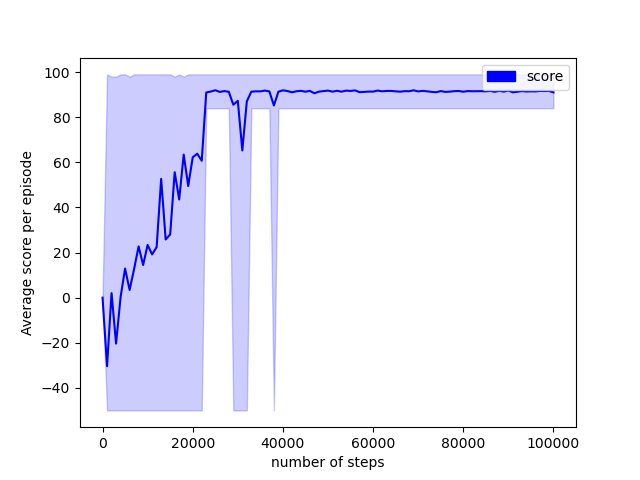
\includegraphics[width=8cm,height=6cm]{./code/performance.png}
	\caption{Q-Learning算法,开启阶梯学习率和经验回放,$\alpha=0.1,\gamma=0.8,replay\_size=100$。}
	\label{performance}
\end{figure}
平均累计奖励随样本训练量的增大而增大,并在平均奖励达到90左右时趋于稳定。模型的最小累计奖励可以维持在85,如果在测试过程中,初始位置从未重置到最坏情况,则可以获得更高的最小奖励,因此最小奖励会略有波动。最终,模型在不同位置的决策结果如下图所示。
\begin{figure}[h!]
	\centering
	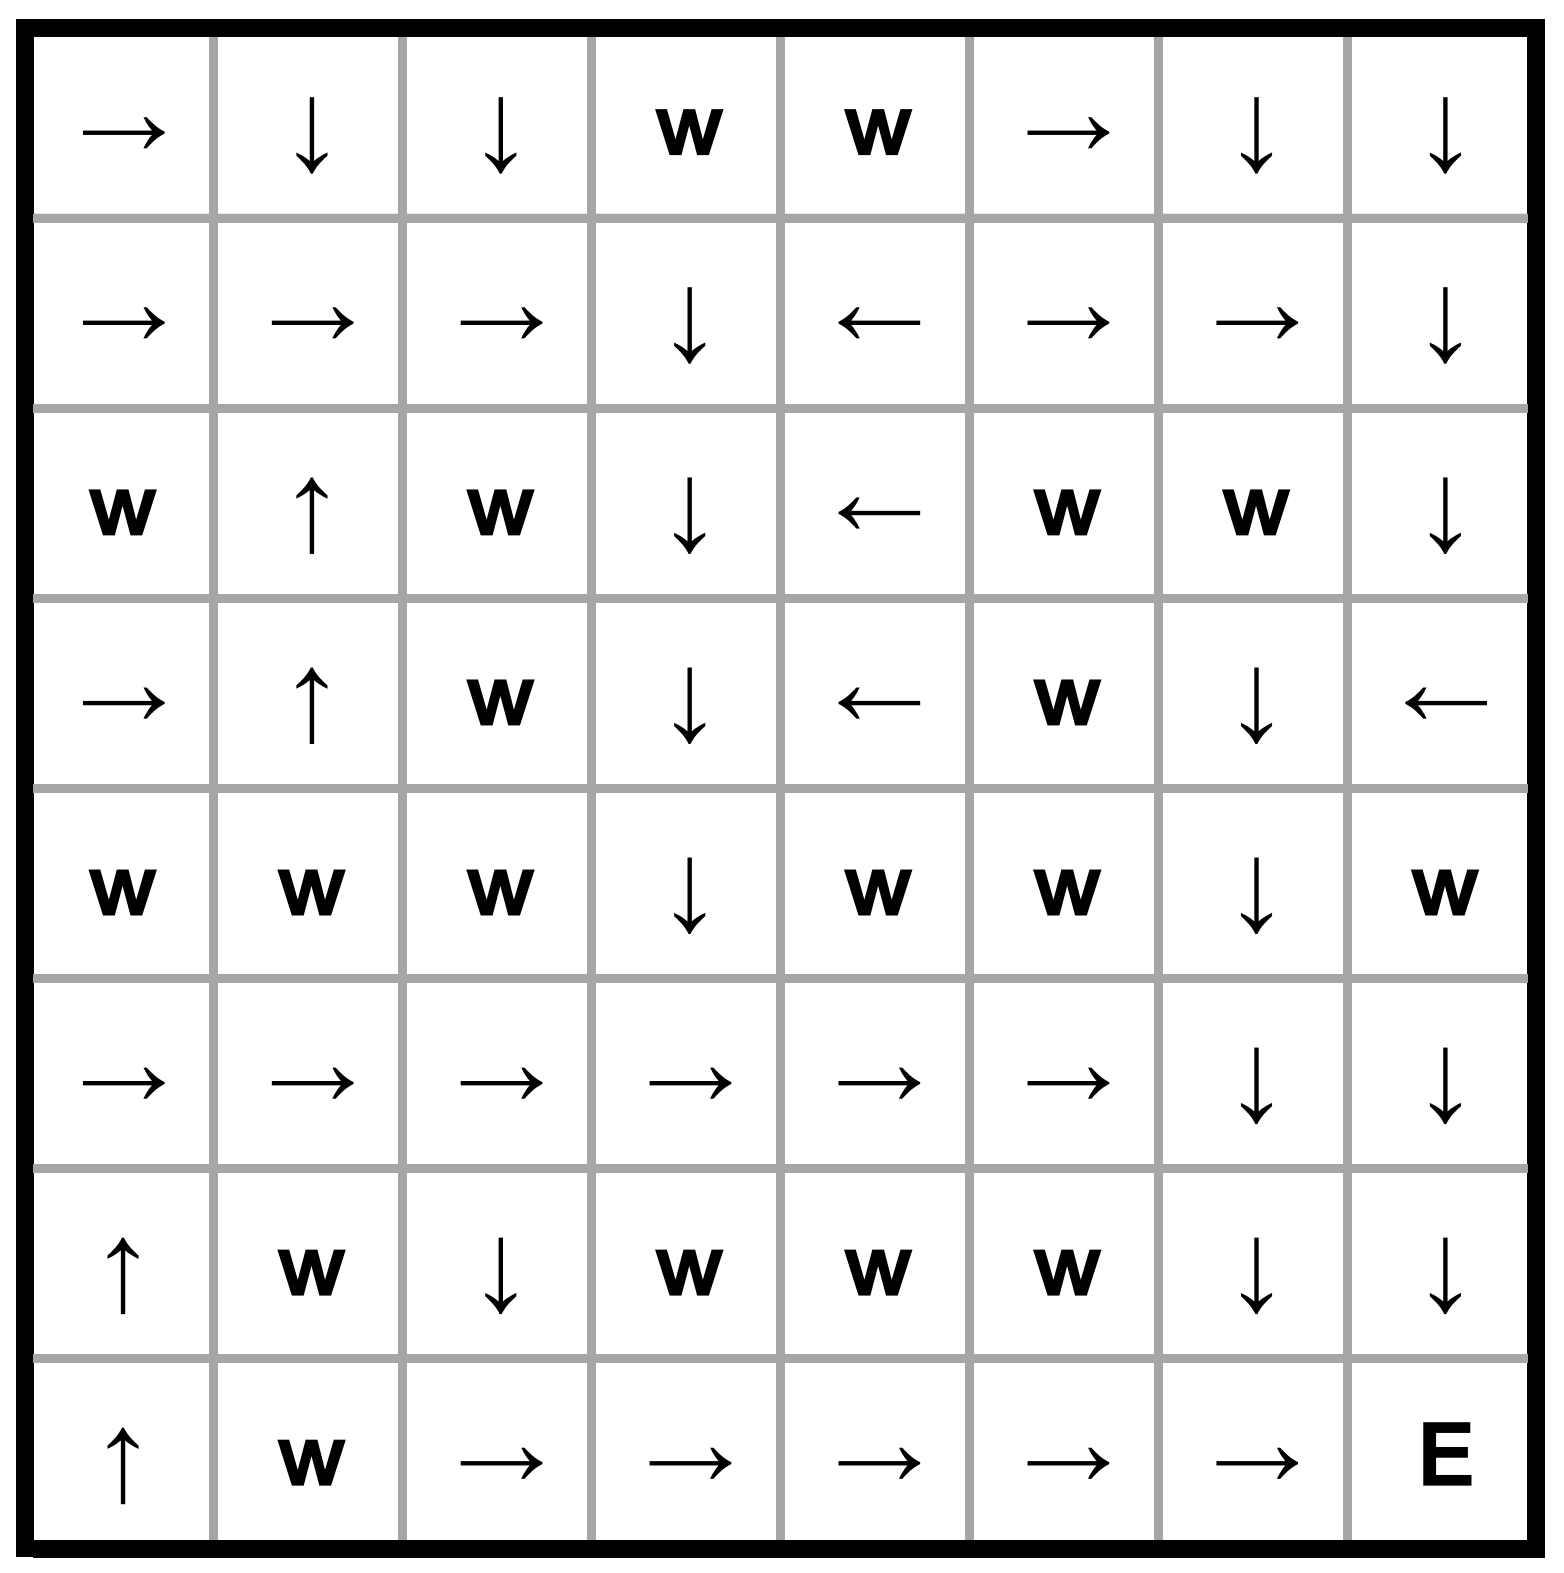
\includegraphics[width=6cm,height=6cm]{./code/result.png}
	\caption{模型最终决策结果}
	\label{performance}
\end{figure}

为了探究经验回放和阶梯学习率的作用,以及每次采样的批大小对实验结果的影响,我依次修改部分参数,进行了如下对比实验:
\begin{figure}[htbp]
	\centering
	\begin{minipage}[t]{0.45\textwidth}
		\centering
		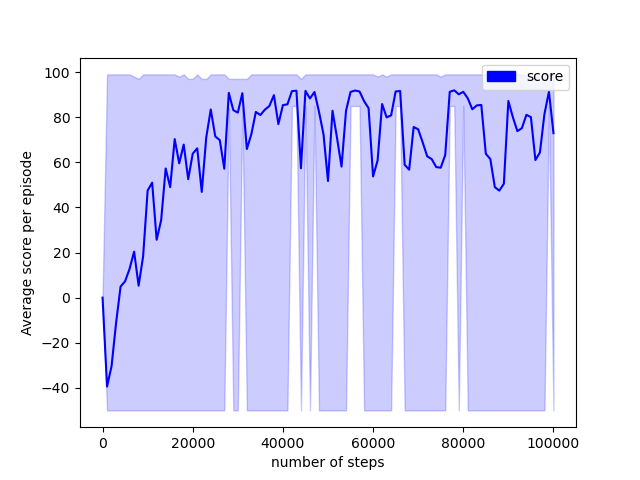
\includegraphics[width=6cm]{code/performance_al=0.1_ga=0.8.png}
		\caption{\tiny 关闭阶梯学习率和经验回放,$\alpha=0.1$,$\gamma=0.8$。}
	\end{minipage}
	\hspace{0.5cm}
	\begin{minipage}[t]{0.45\textwidth}
		\centering
		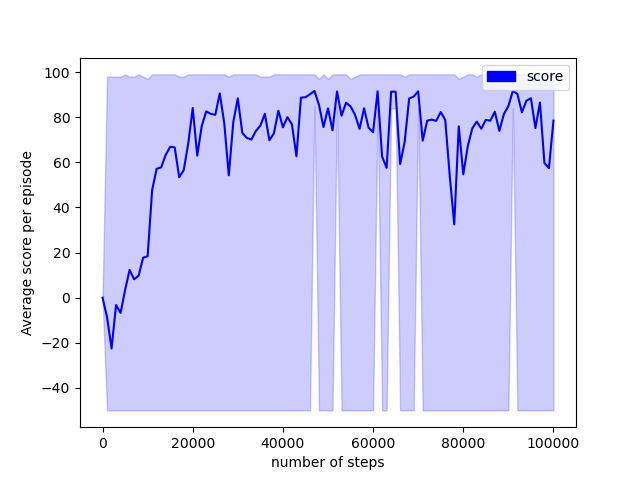
\includegraphics[width=6cm]{code/performance_al=0.1_ga=0.8_rs=100.png}
		\caption{\tiny 关闭阶梯学习率,$\alpha=0.1$,$\gamma=0.8$,$replay\_size=100$。}
	\end{minipage}
	\hspace{0.5cm}
	\begin{minipage}[t]{0.45\textwidth}
		\centering
		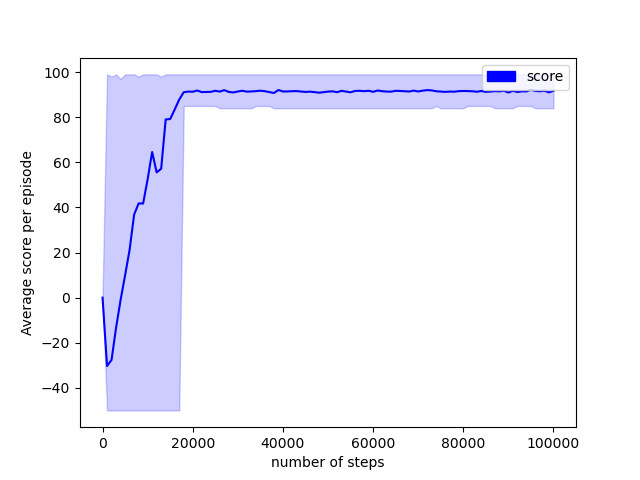
\includegraphics[width=6cm]{code/performance_al=0.1_ga=0.8_laal=T.png}
		\caption{\tiny 关闭经验回放,$\alpha=0.1$,$\gamma=0.8$。}
	\end{minipage}
	\hspace{0.5cm}
	\begin{minipage}[t]{0.45\textwidth}
		\centering
		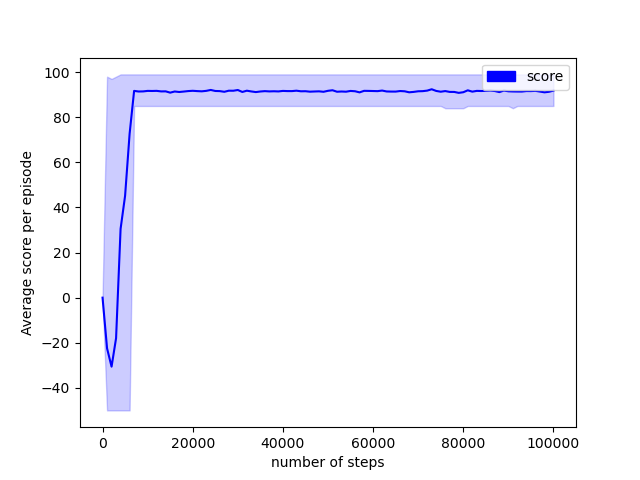
\includegraphics[width=6cm]{code/performance_bs=1.png}
		\caption{\tiny 每次采样后立即更新,开启阶梯学习率和经验回放,$\alpha=0.1$,$\gamma=0.8$,$replay\_size=100$。}
	\end{minipage}
\end{figure}


通过对比实验我们可以发现,快速更新长期回报表 $Q_\pi(s,a)$ 可以显著提高模型的训练速度。此外,阶梯学习率能提高模型的效果和训练速度,并且能够有效稳定我们训练过程。相比之下,在当前参数设置下,经验回放机制似乎没能够提升模型最终的效果,只是略微稳定了训练过程,但是同时也显著降低了训练速度。因此在传统Q-Learning算法中,经验回放也许没能像它在QDN中那样有效。
\section{小结}
\subsection{关于算法本身}
在这次实验中,我发现由于Q-learning算法不依赖专家知识,相较于Dagger算法实现更加方便,并且在gridworld环境中也能取得较好的效果,但是Q-learning需要设置更多的超参数,并且模型的最终效果严重依赖于这些超参数的设置,我们需要在实验过程中不断尝试来选取最优参数设置方案。此外,在本实验中我采用了表格的方式来记录 $Q_\pi$ 值。这种方式在模型收敛后可以取得十分稳定的效果,以至于在模型稳定时的长期回报值 $Q_\pi$ 几乎和理论上的长期回报值完全一致。但在面对“状态-动作”空间较大复杂问题时,往往难以完成训练,因此在面对较为复杂的问题时,利用其他机器学习算法预测 $Q_\pi$ 值可能会更加高效。同时,由于Q-learning使用argmax操作选择动作,因此会略微高估真实 $Q_\pi$ 值,但是由于当前问题比较简单,估计偏差对实验结果的影响较小。
\subsection{关于实验过程}
在实验过程中,我们发现在模型稳定后的最小奖励维持在84,但实际上从迷宫的最远位置到终点仅需15步,经过排查发现这是由游戏结束重置环境时未更新 \texttt{obs} 导致的,在修改代码后终于能够输出正确的结果了。在实验过程中我还发现,在完全随机采样的情况下,只要选取了合适的超参数模型最终依旧可以收敛到最优状态,但是这样训练出来的模型会非常不稳定,在采样数据中存在错误信息时会剧烈抖动。
\end{CJK}
\end{document}
